\documentclass[a4paper]{article}

%% Language and font encodings
\usepackage[english]{babel}
\usepackage[utf8x]{inputenc}
\usepackage[T1]{fontenc}
\usepackage{tikz}

%% Sets page size and margins
\usepackage[a4paper,top=3cm,bottom=2cm,left=3cm,right=3cm,marginparwidth=1.75cm]{geometry}

%% Useful packages
\usepackage{amsmath}
\usepackage{graphicx}
\usepackage[colorinlistoftodos]{todonotes}
\usepackage[colorlinks=true, allcolors=blue]{hyperref}

%% Use APACite
\usepackage{apacite}

%% Use lstlisting
\usepackage{listings}
\usepackage{color}

\usepackage{pgfplots}
\pgfplotsset{compat=1.5}

\usepackage{multicol}

\title{IFT6255 TP1}
\author{Yan AI, Jiechen WU}

\begin{document}
\maketitle

\begin{abstract}
Your abstract.
\end{abstract}

\section{Introduction}
Un système de recherche d’information doit faire 2 opérations de base: l’indexation de documents (et de la requête) et la recherche. 
Il y a certains choix sont possibles pour ces deux opérations. 
Pour l’indexation, on peut choisir à utiliser ou non une stopliste,et un algorithme de stemming.
Pour la recherche, différents modèles peuvent être utilisés :Modèle vectoriel avec la pondération tf*idf , Modèle vectoriel avec la pondération BM25 , Modèle de langue statistique avec le lissage Dirichlet.
 Dans ce devoir,  on profite Indri.  
 Le premier objectif de ce devoir est de tester les différentes options sur une collection de test pour comparer leurs performances. 
 Le deuxième objectif est de comprendre comment un système de RI peut être implanté, en analysant le code de Indri et en le connectant avec une ressource que nous allons  développer nous-mêmes.




\section{Indexation}

\subsection{Stemming}
Nous avons comparé les méthodes du stemming, Porter et Krovetz sans stopliste. Voyez Tableau \ref{tab:porter_vs_krovetz}, pour example. 
cet table montre clairement. n'importe de Porter ou Krovetz ,les méthodes de stemming améliorent évidemment la performance .




\begin{table}[htp]
\centering
\begin{tabular}{|l|l|l|l|l|l|l|}
\hline
Request & Indicator & non-stemming & Porter     & improve & Krovetz    & improve \\ \hline
1-50    & map       & 0.1171       & 0.1538     & 31.34\% & 0.1553     & 32.62\% \\ \hline
        & recall    & 1352/3720    & 1540/3720  & 13.91\% & 1483/3720  & 9.69\%  \\ \hline
        & precision & 1352/48038   & 1540/48062 & 13.85\% & 1483/48210 & 9.30\%  \\ \hline
51-100  & map       & 0.1891       & 0.2383     & 26.02\% & 0.2219     & 17.35\% \\ \hline
        & recall    & 4545/11946   & 5444/11946 & 19.78\% & 5379/11946 & 18.35\% \\ \hline
        & precision & 4545/46496   & 5444/47092 & 18.26\% & 5379/46658 & 17.94\% \\ \hline
101-150 & map       & 0.1765       & 0.1961     & 11.10\% & 0.1982     & 12.29\% \\ \hline
        & recall    & 4129/9873    & 4925/9873  & 19.28\% & 4771/9873  & 15.55\% \\ \hline
        & precision & 4129/50000   & 4925/50000 & 19.28\% & 4771/50000 & 15.55\% \\ \hline
\end{tabular}
\caption{Non-stemming vs Porter vs Krovetz}
\label{tab:porter_vs_krovetz}
\end{table}

\subsection{Stopliste}


\begin{table}[htp]
\centering
\begin{tabular}{|l|l|l|l|l|}
\hline
Request & Indicator & NSTP       & STP        & improve \\ \hline
1-50    & map       & 0.1171     & 0.1135     & -3.07\% \\ \hline
        & recall    & 1352/3720  & 1330/3720  & -1.63\% \\ \hline
        & precision & 1352/48038 & 1330/48038 & -1.63\% \\ \hline
51-100  & map       & 0.1891     & 0.187      & -1.11\% \\ \hline
        & Recall    & 4545/11946 & 4487/11946 & -1.28\% \\ \hline
        & Precision & 4545/46496 & 4487/46496 & -1.28\% \\ \hline
101-150 & map       & 0.1765     & 0.1792     & 1.53\%  \\ \hline
        & Recall    & 4129/9873  & 4149/9873  & 0.48\%  \\ \hline
        & Precision & 4129/50000 & 4149/50000 & 0.48\%  \\ \hline
\end{tabular}
\caption{Non-stopwords vs Stopwords}
\label{nstp_vs_stp}
\end{table}


\subsubsection{La stopliste dans l'indexation vs dans la requête}

Au lieu de inclure la stopliste lorsque l'indexiation (Figure \ref{fig:placement_stp}),
on a un autre choix: Ajoutons la stopliste dans la requête lorsque on exécute IndriRunQuery. En plus, nous avons trouvé que les documents retirés de deux méthode sont totalement identiques.
Alors , on a ajouté le stoplist dans nos indexations, et a trouvé les résultats, comme la table  \ref{nstp_vs_stp}. 

\subsubsection{L'affection de la stopliste}

  selon la table  \ref{nstp_vs_stp} , on trouve que le resultat de non-stoplist est meilleur. 
Generalement, l'elimination des mot de stoplist peut améliorer l'efficacité de IR, mais dans nos essais, la performance n'améliore pas avec le stoplist. 


nous voulions savoir pourquoi.on a trouvé que certaines requêtes ne ont pas marché, comme la \#7 requête, la \#9 requête ......la \#101, la \#106......la \#150 requête . on a observé et a trouvé que toutes les requêtes qui n'avaient pas marché avec des ponctuations. on a essayé d'éliminer lesponctuations de \#7 requête , puis , il a bien marché . Donc, on a éliminé toutes les ponctuations de toutes les requêtes. 


 Alors  , les mots comme U.S. ont devenu les US qui est dans le stoplist.
 Par conséquence,les mots U.S. étaient éliminés, et peut-être  ça a un mauvais effet pour le résultat de valeur de MAP.
 Donc,on a compté la fréquence de mot U.S.dans chaque ensemble  pour savoir bien si les U.S. pouvaiten influencer suffisamment le MAP, comme la table \ref{tab:word_us}. En effet, le résultat de non-stoplist est toujours meilleur . Ensuite, on a remplacé les United States par les U.S. . ça n'a pas  amélioré le resultat. 
 On a aussi essayé de remplacer le U.S. par USA. ça n'améliorepas non plus.voyez la table \ref{us_vs_usa}.  
 On pense que les mots U.S. dans trois ensemble sont une petit quantité de influencer le résultat .

 
 


\begin{table}[htp]
\centering
\begin{tabular}{|l|l|l|l|}
\hline
   & 1-50 & 51-100 & 101-150 \\ \hline
U.S. & 5    & 3      & 11      \\ \hline
\end{tabular}
\caption{La fréquence du mot 'U.S.'}
\label{tab:word_us}
\end{table}

\begin{table}[htp]
\centering
\begin{tabular}{|l|l|l|l|}
\hline
Request & US     & United States & USA    \\ \hline
1-50    & 0.1135 & 0.1117        & 0.1106 \\ \hline
51-100  & 0.187  & 0.1873        & 0.1867 \\ \hline
101-150 & 0.1792 & 0.1763        & 0.1695 \\ \hline
\end{tabular}
\caption{The MAP value after replacement \{US,United States,USA\}}
\label{us_vs_usa}
\end{table}

The map value after replacement of the word 'U.S.' by US/United States/USA

\tikzset{every picture/.style={line width=0.75pt}} %set default line width to 0.75pt

\begin{figure}
\centering
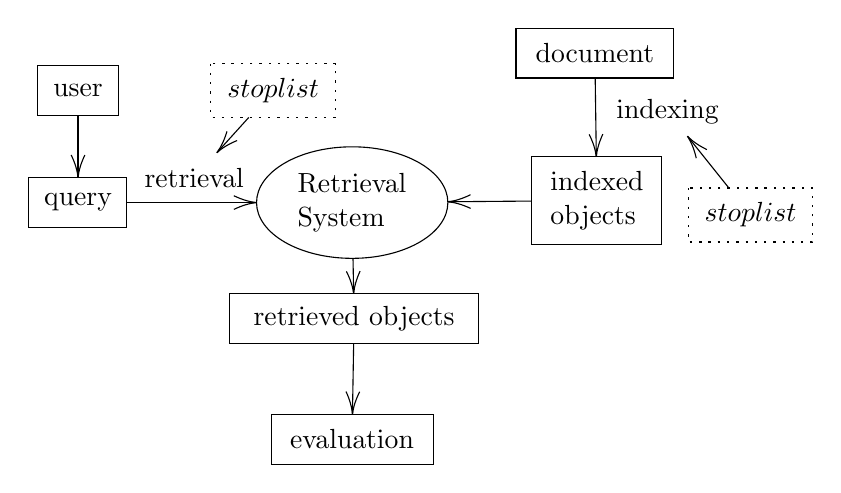
\begin{tikzpicture}[x=0.75pt,y=0.75pt,yscale=-1,xscale=1]
%uncomment if require: \path (0,361); %set diagram left start at 0, and has height of 361

\draw     (24, 107) rectangle (71.53, 131)   ;
\draw (48,119) node  [align=left] {query};
\draw    (180.09, 119) circle [x radius= 46.09, y radius= 26.87]   ;
\draw (180,119) node  [align=left] {Retrieval\\System};
\draw     (266.5, 97) rectangle (329.05, 139)   ;
\draw (298,118) node  [align=left] {indexed\\objects};
\draw     (121, 163) rectangle (241.06, 187)   ;
\draw (181,175) node  [align=left] {retrieved objects};
\draw     (141, 221) rectangle (219.39, 245)   ;
\draw (180,233) node  [align=left] {evaluation};
\draw     (259, 35) rectangle (334.88, 59)   ;
\draw (297,47) node  [align=left] {document};
\draw     (28.5, 53) rectangle (67.69, 77)   ;
\draw (48,65) node  [align=left] {user};
\draw (332,75) node  [align=left] {indexing};
\draw (104,107) node  [align=left] {retrieval};
\draw  [dash pattern={on 0.84pt off 2.51pt}]   (342, 112) rectangle (401.92, 138)   ;
\draw (372,125) node   {$stoplist$};
\draw  [dash pattern={on 0.84pt off 2.51pt}]   (112, 52) rectangle (171.92, 78)   ;
\draw (142,65) node   {$stoplist$};
\draw    (71.53,119) -- (134,119) ;
\draw [shift={(134,119)}, rotate = 180] [color={rgb, 255:red, 0; green, 0; blue, 0 }  ]   (0,0) .. controls (3.31,-0.3) and (6.95,-1.4) .. (10.93,-3.29)(0,0) .. controls (3.31,0.3) and (6.95,1.4) .. (10.93,3.29)   ;

\draw    (266.5,118.27) -- (226.18,118.61) ;
\draw [shift={(226.18,118.61)}, rotate = 359.51] [color={rgb, 255:red, 0; green, 0; blue, 0 }  ]   (0,0) .. controls (3.31,-0.3) and (6.95,-1.4) .. (10.93,-3.29)(0,0) .. controls (3.31,0.3) and (6.95,1.4) .. (10.93,3.29)   ;

\draw    (180.48,145.87) -- (180.79,163) ;
\draw [shift={(180.79,163)}, rotate = 268.98] [color={rgb, 255:red, 0; green, 0; blue, 0 }  ]   (0,0) .. controls (3.31,-0.3) and (6.95,-1.4) .. (10.93,-3.29)(0,0) .. controls (3.31,0.3) and (6.95,1.4) .. (10.93,3.29)   ;

\draw    (180.79,187) -- (180.21,221) ;
\draw [shift={(180.21,221)}, rotate = 270.99] [color={rgb, 255:red, 0; green, 0; blue, 0 }  ]   (0,0) .. controls (3.31,-0.3) and (6.95,-1.4) .. (10.93,-3.29)(0,0) .. controls (3.31,0.3) and (6.95,1.4) .. (10.93,3.29)   ;

\draw    (297.17,59) -- (297.7,97) ;
\draw [shift={(297.7,97)}, rotate = 269.19] [color={rgb, 255:red, 0; green, 0; blue, 0 }  ]   (0,0) .. controls (3.31,-0.3) and (6.95,-1.4) .. (10.93,-3.29)(0,0) .. controls (3.31,0.3) and (6.95,1.4) .. (10.93,3.29)   ;

\draw    (48,77) -- (48,107) ;
\draw [shift={(48,107)}, rotate = 270] [color={rgb, 255:red, 0; green, 0; blue, 0 }  ]   (0,0) .. controls (3.31,-0.3) and (6.95,-1.4) .. (10.93,-3.29)(0,0) .. controls (3.31,0.3) and (6.95,1.4) .. (10.93,3.29)   ;

\draw    (361.6,112) -- (341.6,87) ;
\draw [shift={(341.6,87)}, rotate = 411.34000000000003] [color={rgb, 255:red, 0; green, 0; blue, 0 }  ]   (0,0) .. controls (3.31,-0.3) and (6.95,-1.4) .. (10.93,-3.29)(0,0) .. controls (3.31,0.3) and (6.95,1.4) .. (10.93,3.29)   ;

\draw    (130.24,78) -- (114.86,95) ;
\draw [shift={(114.86,95)}, rotate = 312.14] [color={rgb, 255:red, 0; green, 0; blue, 0 }  ]   (0,0) .. controls (3.31,-0.3) and (6.95,-1.4) .. (10.93,-3.29)(0,0) .. controls (3.31,0.3) and (6.95,1.4) .. (10.93,3.29)   ;


\end{tikzpicture}
\caption{\label{fig:placement_stp} Query time stoplist vs Indexing stoplist}
\end{figure}
  



\section{Chereche}
\subsection{TF-IDF vs BM25 Okapi dans l'Indri}
\subsubsection{Le modèle TF-IDF}
Selon \cite{zhai_notes_2001}, le modèle TF-IDF n'est pas un modèle bien définit. Et dans l'Indri, ce modèle est sur la base de la formule Okapi TF.

On suppose que chaque document est présenté respectivement par un vecteur de la fréquence de terme, $\vec{d} =( x_{1} ,x_{2} ,...,x_{n})$ et $\vec{q} =( y_{1} ,y_{2} ,...,y_{n})$dans cela, n est le montant total des termes.

La formule TF de document:
\[tf_{d}( x) =\frac{k_{1} \cdot x}{x+k_{1}\left( 1-b+b\frac{l_{d}}{l_{C}}\right)}\]

La formule TF de requête:
\[tf_{q}( y) = \cdot\frac{Query\_k_{1} \cdot y}{Query\_k_{1} +y}\]

Le score pour la terme $t_{i}$:
\[score(D,q_{i}) = tf_{d}( x) \cdot tf_{q}( y) \cdot idf^{*}(t_{i})^{2} \]

Après la vérification de la source code de l'Indri, nous confirmons que le modèle TF-IDF dans l'Indri concerne déjà la longueur de document. Et il ressemble beaucoup déjà au modèle BM25.

\subsubsection{Le modèle BM25}
\[dtw=\frac{(k_{1}+1) x}{x+k_{1}\left( 1-b+b\frac{l_{d}}{l_{C}}\right)}\]
\[qtw=\frac{( k_{3} +1) y}{k_{3} +y}\]
\[score(D,q_{i}) =idf(t_{i})\cdot qtw \cdot dtw \]

\begin{itemize}
\item dtw: Document Term Weight Factor
\item qtw: Query Term Weight Factor
\end{itemize}



Par default: Query\_k1 = 1000, k3 = 7

\begin{table}[htp]
\centering
\begin{tabular}{|l|l|l|l|l|l|l|}
\hline
Request & Indicator & TFIDF      & OKAPI      & improve & LM mu=2000 & improve \\ \hline
1-50    & recall    & 1385/3720  & 1460/3720  & 5.42\%  & 1446/3720  & 4.40\%  \\ \hline
        & precision & 1385/48210 & 1460/48210 & 5.42\%  & 1446/48210 & 4.40\%  \\ \hline
        & map       & 0.1135     & 0.1307     & 15.15\% & 0.1415     & 24.67\% \\ \hline
51-100  & recall    & 5241/11946 & 5270/11946 & 0.55\%  & 5257/11946 & 0.31\%  \\ \hline
        & precision & 5241/46658 & 5270/46658 & 0.55\%  & 5257/46658 & 0.31\%  \\ \hline
        & map       & 0.2116     & 0.2191     & 3.54\%  & 0.2163     & 2.22\%  \\ \hline
101-150 & recall    & 4655/9873  & 4802/9873  & 3.16\%  & 4729/9873  & 1.59\%  \\ \hline
        & precision & 4655/50000 & 4802/50000 & 3.16\%  & 4729/50000 & 1.59\%  \\ \hline
        & map       & 0.2017     & 0.2038     & 1.04\%  & 0.1974     & -2.13\% \\ \hline
\end{tabular}
\caption{tfidf vs okapi VS Lm mu=2000}
\label{tab:tfidf-okapi-lm}
\end{table}









\subsection{Modèle de langue statistique dans l'Indri}

On compare la perfomance avec mu differences. 
Au début, 
on a choisi mu=2000, 
ensuite on a séparément examiné les mu, 
comme mu=0,mu=4000,mu=6000,mu=5000,mu=4500,mu=9000, mu=1250 et mu=2500. 


Dans la demande de ce devoir, il ecrit " Modèle de langue statistique avec le lissage Dirichlet (avec le « pseudo-count » mu=2000). " .Donc, on a commencé par mu=2000. 
Ensuite, on voudrait savoir si mu egale 0, qu'est-ce qu'il arrive. On peut trouvet directement dans la table \ref{tab:LM} le resultat qui est vraiment pire. 
Alors, on voudrait savoir que si on ajoute 2000 sur mu=2000, qu'est-ce qu'il arrive. 
Est-ce que ça va changer beaucoup comme mu=0 ?
Quand mu=4000, ça change beaucoup. Mais cet fois, il est mieux que mu=2000.
Ensuit, on voudrait savoir si on ajoute encore 2000 sur mu=4000, qu'est-ce qu'il arrive. 
Est-ce qu'il va continuellement améliorer la performance? Le resultat nous montre losrque mu=6000 ,la performance est presque pareil de mu=2000. 
Donc, on a testé mu=5000, le resultat est mieux que mu=6000.
on a testé mu=4500, et mu=4500 et mu=5000 sont similaire.
Généralement, il est possible que mu=1250 ou mu=2000 ou mu=2500 ou mu=4000, la performance est meilleur. on avait déjà fait les tests de mu=2000 et mu=4000. on a fait les tests de mu=1250 et mu=2500.
A la fin, on a essayé de mu=9000  et mu=0 pour voir dans la situation extrême ,qu'est-ce qu'il arrive.
Tous les résultats est montré dans la table \ref{tab:LM}.






\begin{table}[htp]
\centering
\begin{tabular}{|l|l|l|l|l|l|l|l|l|}
\hline
Req & Ind & LM $\mu$2000 & LM $\mu$0    & imp\%  & LM $\mu$1250 & imp\% & LM $\mu$2500 & imp\% \\ \hline
1-50    & rec    & 1446/3720  & 672/3720   & -53.53 & 1441/3720  & -0.35 & 1451/3720  & 0.35  \\ \hline
        & prec & 1446/48210 & 672/48210  & -53.53 & 1441/48210 & -0.35 & 1451/48210 & 0.35  \\ \hline
        & map       & 0.1415     & 0.0163     & -88.48 & 0.1404     & -0.78 & 0.1415     & 0.00  \\ \hline
51-100  & rec    & 5257/11946 & 3188/11946 & -39.36 & 5203/11946 & -1.03 & 5286/11946 & 0.55  \\ \hline
        & prec & 5257/46658 & 3188/46658 & -39.36 & 5203/46658 & -1.03 & 5286/46658 & 0.55  \\ \hline
        & map       & 0.2163     & 0.0865     & -60.01 & 0.2172     & 0.42  & 0.216      & -0.14 \\ \hline
101-150 & rec    & 4729/9873  & 852/9873   & -81.98 & 4635/9873  & -1.99 & 4731/9873  & 0.04  \\ \hline
        & prec & 4729/50000 & 852/50000  & -81.98 & 4635/50000 & -1.99 & 4731/50000 & 0.04  \\ \hline
        & map       & 0.1974     & 0.0063     & -96.81 & 0.1936     & -1.93 & 0.1984     & 0.51  \\ \hline
        &           &            &            &          &            &         &            &         \\ \hline
        &           &            &            &          &            &         &            &         \\ \hline
Req & Ind & LM $\mu$2000 & LM $\mu$4000 & imp\%  & LM $\mu$4500 &         & LM $\mu$5000 &         \\ \hline
1-50    & rec    & 1446/3720  & 1453/3720  & 0.48   & 1449/3720  & 0.21  & 1449/3720  & 0.21  \\ \hline
        & prec & 1446/48210 & 1453/48210 & 0.48   & 1449/48210 & 0.21  & 1449/48210 & 0.21  \\ \hline
        & map       & 0.1415     & 0.1398     & -1.20  & 0.1391     & -1.70 & 0.1378     & -2.61 \\ \hline
51-100  & rec    & 5257/11946 & 5301/11946 & 0.84   & 5281/11946 & 0.46  & 5279/11946 & 0.42  \\ \hline
        & prec & 5257/46658 & 5301/46658 & 0.84   & 5281/46658 & 0.46  & 5279/46658 & 0.42  \\ \hline
        & map       & 0.2163     & 0.2127     & -1.66  & 0.2114     & -2.27 & 0.2104     & -2.73 \\ \hline
101-150 & rec    & 4729/9873  & 4764/9873  & 0.74   & 4764/9873  & 0.74  & 4766/9873  & \textbf{0.78}  \\ \hline
        & prec & 4729/50000 & 4764/50000 & 0.74   & 4764/50000 & 0.74  & 4766/50000 & \textbf{0.78}  \\ \hline
        & map       & 0.1974     & 0.1997     & 1.17   & 0.1999     & 1.27  & 0.2        & \textbf{1.32}  \\ \hline
        &           &            &            &          &            &         &            &         \\ \hline
        &           &            &            &          &            &         &            &         \\ \hline
Req & Ind & LM $\mu$2000 & LM $\mu$6000 &          & LM $\mu$9000 &         &            &         \\ \hline
1-50    & rec    & 1446/3720  & 1446/3720  & 0.00   & 1429/3720  & -1.18 &            &         \\ \hline
        & prec & 1446/48210 & 1446/48210 & 0.00   & 1429/48210 & -1.18 &            &         \\ \hline
        & map       & 0.1415     & 0.137      & -3.18  & 0.1351     & -4.52 &            &         \\ \hline
51-100  & rec    & 5257/11946 & 5257/11946 & 0.00   & 5201/11946 & -1.07 &            &         \\ \hline
        & prec & 5257/46658 & 5257/46658 & 0.00   & 5201/46658 & -1.07 &            &         \\ \hline
        & map       & 0.2163     & 0.2081     & -3.79  & 0.2036     & -5.87 &            &         \\ \hline
101-150 & rec    & 4729/9873  & 4756/9873  & 0.57   & 4702/9873  & -0.57 &            &         \\ \hline
        & prec & 4729/50000 & 4756/50000 & 0.57   & 4702/50000 & -0.57 &            &         \\ \hline
        & map       & 0.1974     & 0.1999     & 1.27   & 0.1976     & 0.10  &            &         \\ \hline
\end{tabular}
\caption{LM avec mu differences}
\label{tab:LM}
\end{table}

Généralement, la valeur map c'est le metric on va utiliser. Mais on observe aussi la situation que mu2500 et mu2000 nous donnent la même map néanmoins les différents rappels et précision sur les requêtes 1-50. 

on peut directement regarder les changements parmi les mu différents .  La permanence avec mu=0 est le pire. Et pour chaque ensemble de données, il y a un mu concordé qui donne le meilleur performance. 



\begin{itemize}
\item Requête 1-50: mu=2500
\item Requête 51-100: mu=2000
\item Requête 101-150: mu=5000
\end{itemize}
\begin{figure}
\centering
\begin{multicols}{2}
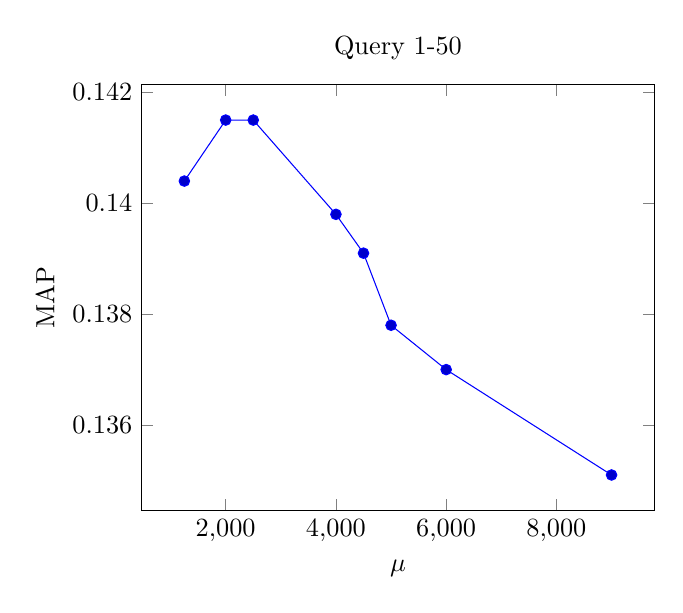
\begin{tikzpicture}[thick,scale=0.95]
\begin{axis}[
title= Query 1-50,
xlabel= {$\mu$},
ylabel= MAP,
y tick label style={
        /pgf/number format/.cd,
            precision=3
    }]
\addplot table[x=mu,y=MAP] {
mu   MAP
1250 0.1404
2000 0.1415
2500 0.1415
4000 0.1398
4500 0.1391
5000 0.1378
6000 0.137
9000 0.1351
};
\end{axis}
\end{tikzpicture}

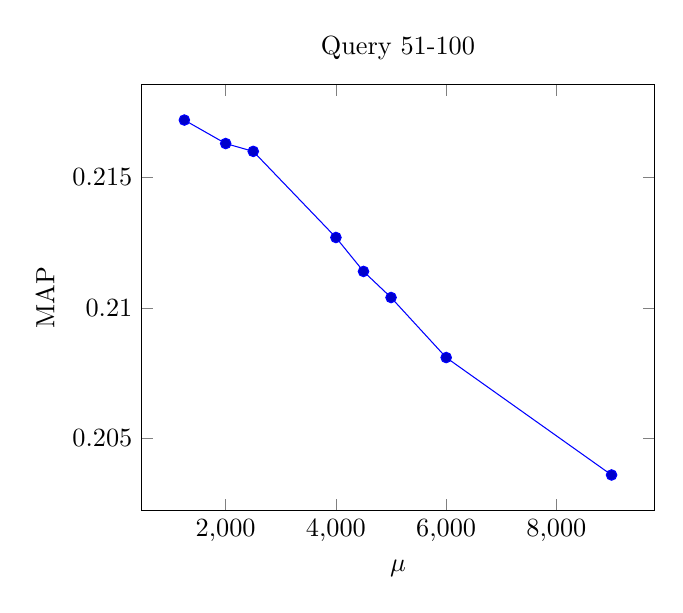
\begin{tikzpicture}[thick,scale=0.95]
\begin{axis}[
title= Query 51-100,
xlabel= {$\mu$},
ylabel= MAP,
y tick label style={
        /pgf/number format/.cd,
            precision=3
    }]
\addplot table[x=mu,y=MAP] {
mu   MAP
1250 0.2172
2000 0.2163
2500 0.216
4000 0.2127
4500 0.2114
5000 0.2104
6000 0.2081
9000 0.2036
};
\end{axis}
\end{tikzpicture}

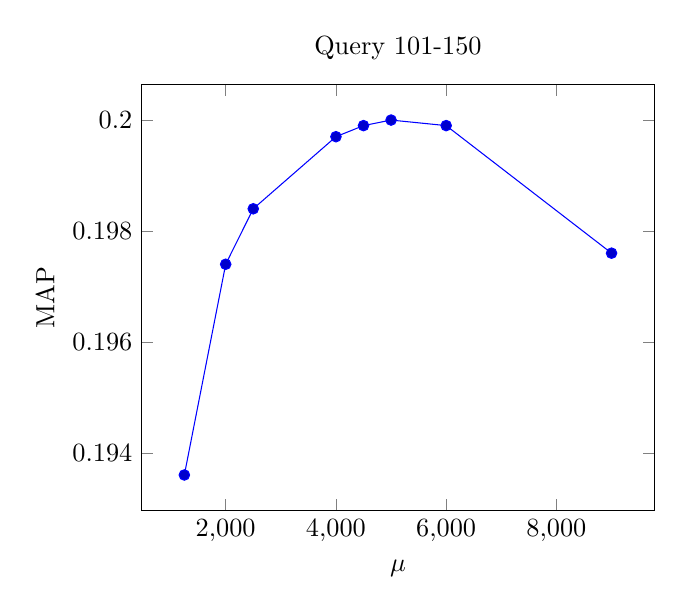
\begin{tikzpicture}[thick,scale=0.95]
\begin{axis}[
title= Query 101-150,
xlabel= {$\mu$},
ylabel= MAP,
y tick label style={
        /pgf/number format/.cd,
            precision=3
    }]
\addplot table[x=mu,y=MAP] {
mu   MAP
1250 0.1936
2000 0.1974
2500 0.1984
4000 0.1997
4500 0.1999
5000 0.2
6000 0.1999
9000 0.1976
};
\end{axis}
\end{tikzpicture}
\end{multicols}
\end{figure}

Observons la formule Dirichilet:
\begin{equation}
P_{Dir}(w_i|D)=\frac{tf(w_i,D)+\mu P_{ML}(w_i|C)}{|D|+\mu}
\end{equation}

Quand le mu=0, il n'y a pas de lissage. Il donne de la mouvaise performance. Puis, si le mu est assez grand, on ignore l'influence de chaque document. Il donne de la mouvais performance aussi.  












\section{Expansion de requête}
\subsection{Expansion locale de requête}
Un des problèmes en RI est que les requêtes sont souvent trop courtes, et ne contiennent
pas tous les mots importants. Une approche courante est de faire l’expansion de requête,
en y ajoutant des mots extraits de documents de feedback.
Une des implantations est Relevance model, implanté dans Indri. On  utilise ce modèle pour étendre la requête. 
Au début ,on a utilisé 10 documents et extraire
10 termes. après, on a varié ces nombres pour voir les effets.
 
  on a divisé en 5 groupes ,
 
  comme:
  
  1. 10 documents et extraire 10 termes;
  
  2. 5 documents et extraire 10 termes;
  
  3. 10 documents et extraire 5 termes;
 
  4. 5 documents et extraire 5 termes;
  
  5. 20 documents et extraire 20 termes;
  
 la table  \ref{tab:comp_fb} montre la comparaison de 5 groupes.
  
  En effet ,Dans nos 5 groupe , la performance de première groupe qu'on utilise 10 documents et extraire 10 termes est le meilleur . Dans l'ensemble, cet méthode peut améliorer la performance .  Mais Les 5 groupes n'améliorent pas sur le premier ensemble.

\begin{table}[htp]
\centering
\begin{tabular}{|l|l|l|l|l|l|l|l|l|}
\hline
Req & Ind & Baseline    & fbD10,fbT10 & imp\%  & fbD5,fbT10  & imp\% & fbD10,fbT5 & imp\%  \\ \hline
1-50    & rec    & 1451/3720  & 1790/3720   & 23.36  & 1813/3720   & 24.95 & 1764/3720  & 21.57  \\ \hline
        & prec & 1451/50000 & 1790/50000  & 23.36  & 1813/50000  & 24.95 & 1764/50000 & 21.57  \\ \hline
        & map       & 0.1415     & 0.1298      & -8.27  & 0.1399      & -1.13 & 0.1171     & -17.24 \\ \hline
51-100  & rec    & 5286/11946 & 6086/11946  & 15.13  & 6105/11946  & 15.49 & 5956/11946 & 12.67  \\ \hline
        & prec & 5286/50000 & 6086/50000  & 15.13  & 6105/50000  & 15.49 & 5956/50000 & 12.67  \\ \hline
        & map       & 0.216      & 0.2636      & 22.04  & 0.2627      & 21.62 & 0.2559     & 18.47  \\ \hline
101-150 & rec    & 4731/9873  & 5707/9873   & 20.63  & 5695/9873   & 20.38 & 5453/9873  & 15.26  \\ \hline
        & prec & 4731/50000 & 5707/50000  & 20.63  & 5695/50000  & 20.38 & 5453/50000 & 15.26  \\ \hline
        & map       & 0.1984     & 0.2492      & 25.60  & 0.2481      & 25.05 & 0.2378     & 19.86  \\ \hline
        &           &            &             &          &             &         &            &          \\ \hline
        &           &            &             &          &             &         &            &          \\ \hline
Req & Ind & Baseline    & fbD5,fbT5   & imp\%  & fbD20,fbT20 & imp\% &            &          \\ \hline
1-50    & rec    & 1451/3720  & 1748/3720   & 20.47  & 1759/3720   & 21.23 &            &          \\ \hline
        & prec & 1451/50000 & 1748/50000  & 20.47  & 1759/50000  & 21.23 &            &          \\ \hline
        & map       & 0.1415     & 0.1217      & -13.99 & 0.1375      & -2.83 &            &          \\ \hline
51-100  & rec    & 5286/11946 & 6017/11946  & 13.83  & 5971/11946  & 12.96 &            &          \\ \hline
        & prec & 5286/50000 & 6017/50000  & 13.83  & 5971/50000  & 12.96 &            &          \\ \hline
        & map       & 0.216      & 0.2537      & 17.45  & 0.2598      & 20.28 &            &          \\ \hline
101-150 & rec    & 4731/9873  & 5416/9873   & 14.48  & 5943/9873   & 25.62 &            &          \\ \hline
        & prec & 4731/50000 & 5416/50000  & 14.48  & 5943/50000  & 25.62 &            &          \\ \hline
        & map       & 0.1984     & 0.2356      & 18.75  & 0.2645      & 33.32 &            &          \\ \hline
        &           &            &             &          &             &         &            &          \\ \hline
\end{tabular}
\caption{comparation-fb}
\label{tab:comp_fb}
\end{table}

\subsection{Expansion global de requête}
Une autre approche dite globale est d’extraire des relations entre les termes sur
toute la collection, et appliquer ces relations sur la requête donnée pour l’étendre. On a implanté ce processus d’expansion et deux étapes. 

\subsubsection{Extraction de relation entre les termes}
Nous avons écrit un programme pour extracter les relation dans la collection de test. L'idée est simple, on met une fenêtre qui a la taile est $distance+1$. Et chaque foi, on glisse la fenêtre arrière un mots, au même temps, on accumule le cooccurrences de fréquence entre le nouveau mot dans la fenêtre  et chaque mot existe déjà dans celle. 

Les deux mesures pour calculer le score de mot de relation, les formules est:
\begin{align}
P(t_j|t_i)&=\frac{\#cooc(t_i,t_j)}{\sum_{t_k}{\#cooc(t_i,t_k)}} \label{eq:ptji1} \\
&=\frac{\#cooc(t_i,t_j)}{2T\cdot freq(t_i)} \label{eq:ptji2} \\
PMI(t_i,t_j)&=\frac{P(t_i,t_j)}{P(t_i)P(t_j)} \\
&=\frac{\#cooc(t_i,t_j)\cdot \sum_{t_j}\sum_{t_i}\#cooc(t_i,t_j)}
{\sum_{t_k}{\#cooc(t_i,t_k)}\sum_{t_k}{\#cooc(t_j,t_k)}} \\
&=\frac{\#cooc(t_i,t_j)\cdot N \cdot 2T}
{freq(t_i)\cdot 2T\cdot freq(t_i)\cdot 2T } \\
&=\frac{\#cooc(t_i,t_j)}{2T\cdot freq(t_i)}\cdot \frac{N}{freq(t_j)} \label{eq:ptji3}
\end{align}

Ici, $T$ représente la distance de relation. De l’équation \ref{eq:ptji1} à l'équation \ref{eq:ptji2}, on suppose que ce mot n'affiche pas ce mot affiche pas au début ou à la fin de chaque fiche. Il y a existe toujours $2T\cdot freq(t_i)$ relations pour chaque mot, celles qui contient le mot il même. Comme cela, on peut faciliter notamment le calcul. Et puis, si on insère l'équation \ref{eq:ptji2} dans l'équation \ref{eq:ptji3}, on peut voir que :
\[PMI(t_i,t_j)=P(t_j|t_i)\cdot \frac{N}{freq(t_j)}\]

Cela signifie que on peut toujours calculer le PMI en base de $P(t_j|t_i)$ en temps constant si on garde la $freq(t_j)$ dans la liste. En effet, N fait rien ici. Si on veut, on peut encore la simplifier:
\[PMI(t_i,t_j)\propto  \frac{P(t_j|t_i)}{freq(t_j)}\]

Normalement, la fonction log peut aussi être utilisé ici. La fonction log ne change pas les termes reliés que on choisit, mais il changera les pondérations finales des termes reliés dans la requête dans l'Indri.

Après de compter la cooccurrence pour chaque relation, on filtre la liste et calcule le score au même temps. Puis on choisit l0 termes les plus reliés et enregistre la liste pour la 2ème étape.

Avec la seuil 5, il nous prends 30 mins pour obtenir la collection de relation pour le corpus.

\subsubsection{Utiliser les relations dans la RI}

On crée nos requête dans la forme de l'Indri avec le score $P(t_j|t_i)$ que on calcule dans l'étape précédente. Par exemple: la requête d'orinale est "Cases Pending". Dans notre liste de collection de relation, on repère les 10 mots reliés le plus au "cases" et 10 mots reliés au "pending" et leurs score. On prend 3 mots reliés pour chaque, à titre d'exemple. Et supposons $\lambda=0.7$
\begin{lstlisting}
   cases   => {court:0.45, fedral:0.35, pending:0.15}
   pending => {year:0.4 court:0.3, law:0.25}
\end{lstlisting}
Ensuite, on fait notre requête:
\begin{lstlisting}
   #weight( 0.7 #combine (antritrust cases pending) + 0.3 #weight ( 
   0.45 court 0.35 fedral 0.15 pending 0.4 year 0.3 court 0.25 law))
\end{lstlisting}

Donc on calcul la probabilité de chaque terme relié en donnant la requête.
\begin{align*}
z&=(0.45+0.35+0.15+0.4+0.3+0.25)/2 = 0.95 \\
P(court|Q) &= 0.7*0 + 0.3* (0.45*0.5 + 0.3*0.5)/z = 0.118 \\
P(fedral|Q) &= 0.7*0 + 0.3*0.35*0.5/z = 0.055 \\
P(pending|Q) &= 0.7*0.5 + 0.3* 0.15*0.5/z = 0.374 \\
p(year|Q) &= 0.7*0 + 0.3*0.4*0.5/z = 0.063 \\
p(law|Q) &= 0.7*0 + 0.3*0.25*0.5/z = 0.039
\end{align*}


Selon l'équation donnée, c'est une situation idéale. Étant donné qu’on ne garde que les 10 premiers termes les plus reliés, cet élément n’est pas une probabilité dans le sens strict, le $\sum_{t_j}{P(t_j|t_i)}<1$. Est c'est aussi pourquoi nous mettons un $z$ comme normalisateur. En fait, l'Indri va faire sa job pour nous. 
\[P( t_{j}|Q) =\lambda P_{ML}( t_{j} |Q) +( 1-\lambda )\sum _{t_{i} \in Q} P( t_{j} | t_{i}) P_{ML}( t_{i} | Q)\]

\begin{table}[htp]
\centering
\begin{tabular}{|l|l|l|l|l|l|l|}
\hline
Request & Indicator & Baseline       & COOC & improve & PMI        & improve  \\ \hline
1-50    & recall    & 1451/3720      & 1531/3720        & 5.51\%  & 1516/3720  & 4.48\%   \\ \hline
        & precision & 1451/48210     & 1531/49002       & 3.81\%  & 1516/49002 & 2.79\%   \\ \hline
        & map       & 0.1415         & 0.1309           & -7.49\% & 0.1117     & -21.06\% \\ \hline
51-100  & recall    & 5286/11946     & 5458/11946       & 3.25\%  & 5467/11946 & 3.42\%   \\ \hline
        & precision & 5286/46658     & 5458/50000       & -3.65\% & 5467/50000 & -3.49\%  \\ \hline
        & map       & 0.216          & 0.2229           & 3.19\%  & 0.2244     & 3.89\%   \\ \hline
101-150 & recall    & 4731/9873      & 4982/9873        & 5.31\%  & 4709/9873  & -0.47\%  \\ \hline
        & precision & 4731/50000     & 4982/50000       & 5.31\%  & 4709/50000 & -0.47\%  \\ \hline
        & map       & 0.1984         & 0.2048           & 3.23\%  & 0.188      & -5.24\%  \\ \hline
\end{tabular}
\caption{Fréquence de co-occurrence relative vs PMI}
\label{tab:esp_glo}
\end{table}
\bibliographystyle{apacite}
\bibliography{sample,IR}

\end{document}